\documentclass[twocolumn]{article}
\usepackage{caption}
\usepackage[utf8]{inputenc}
\usepackage{amsmath}
\usepackage[margin=1in]{geometry}
\usepackage{changepage}
\usepackage{titling}
\usepackage{ragged2e}
\usepackage{abstract}
\usepackage{enumitem}
\usepackage{graphicx}
\usepackage{hyperref}
\renewcommand{\thesection}{\Roman{section}}
\renewcommand{\thesubsection}{(\roman{subsection})}
\renewcommand{\thesubsubsection}{\thesubsection.\arabic{subsubsection}}
\setlength\parindent{5pt}
\setlength{\columnsep}{1cm}

\begin{document}

\twocolumn[
\begin{@twocolumnfalse}
\title{\Large{\textbf{Optical Pumping of $Rb^{85}$ and $Rb^{87}$}}}
\author{Herbert D. Ludowieg}
\setlength{\droptitle}{-0.65in}
\maketitle
\begin{onecolabstract}
\justify
Optical Pumping is a spectroscopical method that was developed in the 1950's 
and has been a very accurate method to determine spectroscopical properties of 
certain materials. In this experiment the following were determined: the 
individual g-factors, nuclear spins, cross sectional area and ratio of the 
periods. For $Rb^{85}$ the g-factor and nuclear spin were found to be: 
0.3260 $\pm$ 0.0005 and 2.571 respectively. For $Rb^{87}$ they were found to 
be: 0.482 $\pm$ 0.001 and 1.576 respectively. The cross-sectional area and 
ratio of the periods were found to be: 1.8$\times10^{-16}$ $\pm$ 
0.3$\times10^{-16}$ and 1.44 $\pm$ 0.05 respectively.
\\
\end{onecolabstract}
\end{@twocolumnfalse}]

\section{Introduction}
Optical Pumping is a spectroscopical method developed in 1950 by Alfred 
Kastler, whom received the Nobel Prize in physics in 1966 for his discovery. 
This method is one in which photons are utilized to create population 
differences of electronic excited and ground states. So the meaning and general 
concept is in the name itself.
\\
Under startdard conditions the population difference required to carry out 
experiments is not possible because from statistical mechanics at thermal 
equilibrium we have an equal number of electrons that rise and fall from 
excitation levels. Due to this, they tend to cancel each others effects and 
no net population differences can be detected. This is also the basis of lasers 
where, a population difference needs to be created so that photons can be 
spontaneously emmitted by the lasing medium.
\\
For this experiment the equipment that is being used is provided by TeachSpin 
and consists of an Radio Frequency (RF) discharge lamp, Interference Filter, 
Polarizers, Quarter Wave plate, absorption cell, optical detector, three sets 
of magnetic coils in a Helmholtz configuration and a RF magnetic coil. The 
sample is a Rubidium glass bulb that contains neon gas with a pressure of 
approximately 0.04 atm pressure. The presence of the neon gas is important as 
its spherical symmetry will reduce the interactions between the Rubidium atoms 
and the outside environment. They will act as a buffer gas.
\\
Optical Pumping is a process in which has had much applicability in solid state 
and liquid state physics. However, we will only be dealing with a gas since at 
the solid and liquid phases the interactions between the neighboring atoms 
increases thus broadening the energy levels \cite{ref:1}.

\section{Theory}
\subsection{Structure of alkali atoms}
In the experiment described in this paper we will be studying the absorption 
and emission from Rubidium isotopes (85 and 87) which are alkali atoms. As such the electronic structure of Rubidium is as such,
\begin{equation*}
1s^22s^22p^63s^23p^63d^104s^24p^65s
\end{equation*}
Where we can show the shorthand version as,
\begin{equation*}
[Kr]5s
\end{equation*}
\center
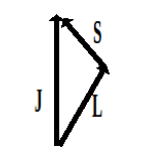
\includegraphics[width=0.3\linewidth]{pictures/electron-angular-momentum.png}
\captionof{figure}{\textit{Coupling of angular momentum in an electron 
\cite{ref:3}.\\}}
\label{fig:1}
\justify
Where, the superscripts show the number of electrons contained in each of the 
electronic shells. Since the only valence electron is in the 5s shell we can 
consider the atom to bev consisting of only one electron. This electron much 
like with other 
electrons can be described by means of the total angular momentum of the 
electron $\vec{J}$ where it is made up of components $\vec{S}$ and 
$\vec{L}$. Which, represent the spin angular momentum and orbital angular 
momentum respectively. The vectors are shown on figure \ref{fig:1}
\\
Since, these components are vectors we can represent the total angular momentum 
as such,
\begin{equation}
\vec{J} = \vec{S}+\vec{L}
\label{eqn:1}
\end{equation}
\justify
Where, for an alkali atom in the ground state the value of $\vec{L}$ is zero 
from the quantum numbers associated with the orbital shell and the value of 
$\vec{S}$ will be 1/2. So, this gives rise to a total angular momentum of 1/2.
\\
As it will later become apparent, we will display some of the energy levels in 
the notation $^{2s+1}L_J$. Where, all of the values are those taken from 
equation \ref{eqn:1}. To represent the ground state of an alkali atom we can 
write it with the formatting $^{2}S_{1/2}$. Since the value of $\vec{L}$ is 
zero by convention we write it as the letter S. Where it to be 1 we would write 
in P and so on.
\\
If the electron were to be in a P state it would be able to have an angular 
momentum of $\vec{L}\pm\vec{S}$ and would take on the representations 
$^{2}P_{1/2}$ and $^{2}P_{3/2}$. Due to the difference in angular momentum the 
energy levels would have different energies. This arises due to the spin-orbit 
coupling of the angular momentum vectors \cite{ref:4}.
\center
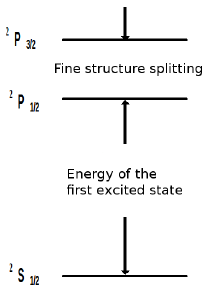
\includegraphics[width=0.5\linewidth]{pictures/energy-levels.png}
\captionof{figure}{\textit{Pictoral representation of the energy difference in the fine structure. Not to scale \cite{ref:3}.}}
\label{fig:2}
\justify
So far, we have been ignoring the effects of the nucleus to make the theory 
easier. However, this will not go on any longer. We will now consider the 
hyperfine splitting of the electron angular momenta. This arises from the 
spin-spin coupling where for the fine structure we had the spin-orbit coupling. 
\\
The spin-spin coupling is due to the magnetic dipole moment of both the proton 
and electron. Now, it should be noted, that the magnetic dipole moment of the 
proton is much smaller than that compared to the electron. The dipole momenta 
can be given as the following.
\begin{equation}
\begin{aligned}
\vec{\mu_p} &= \frac{g_pe}{2m_p}\vec{S_p}
\qquad
\vec{\mu_e} &= -\frac{e}{m_e}\vec{S_e}
\label{eqn:2}
\cite{ref:4}
\end{aligned}
\end{equation}
Where, the p and e represent the proton and electron values respectively, $g_p$ and $g_e$ are the respective g-factors of value 5.59 and 2.00 and $\vec{S}$ 
represents the respective angular spin. Using derivations outlined in reference 
\cite{ref:4} we can get to an expression for the difference in energy of the 
two states with different angular momenta. The equation is as such.
\begin{equation}
\Delta E = \frac{4g_p\hbar}{3m_pm_e^2c^2r^4}
\label{eqn:3}
\cite{ref:4}
\end{equation}
\begin{figure*}
\begin{minipage}[t]{0.46\linewidth}
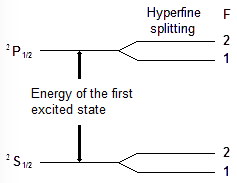
\includegraphics[width=\linewidth]{pictures/hyperfine-splitting.png}
\caption{\textit{Hyperfine splitting energy diagram for I = 3/2 particle 
\cite{ref:3}}}
\label{fig:3}
\end{minipage}
\begin{minipage}[t]{0.46\linewidth}
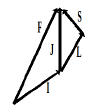
\includegraphics[width=0.3\linewidth]{pictures/hyperfine-vectors.png}
\caption{\textit{Hyperfine coupling in an alkali atom \cite{ref:3}}}
\label{fig:4}
\end{minipage}
\end{figure*}
Where, c is the speed of light and r is the radius of the atom. In the 
reference they are making an example to a hydrogen atom with r equal to a 
(Bohr's atomic radius). This derivation can still be generalized to our use as 
we are dealing with an atom that can be approximated to be one that is like a 
hydrogen atom. Where we can also make the relation with the frequency as such.
\begin{equation}
\nu = \frac{\Delta E}{h}
\label{eqn:4}
\cite{ref:4}
\end{equation}
Where the Hamiltonian is as such.
\begin{equation}
H=ha\vec{I}\cdot\vec{J}
\label{eqn:5}
\cite{ref:3}
\end{equation}
Usually the energy difference between these two levels is very small and one 
can cause transitions in the hyperfine structure with an RF wave. A pictoral 
representation of the coupling of the magnetic dipole moment spins is shown on 
figure \ref{fig:4}. Where a rough enegy separation schematic is given in figure 
\ref{fig:3}. As is clearly seen the energy that is required to jump from one 
energy level to the next is muche greater than that required to make the 
transition in the hyperfine structure. Later we will discuss the implications 
of this with respect to optical pumping.
\\
However next we will show another form of splitting where all of the degenerate 
energy levels of the electronic energy level diagram are split.
\subsection{Interaction of an alkali atom with a magnetic field}
This interaction is better known as the Zeeman effect and the general premise 
behind this effect is that by applying a magnetic field to an atom we can 
further split the degenerate energy levels according to their angular momenta.
\\
In the Zeeman effect there are three main regions that are to be considered: 
weak field, intermediate and Strong field effects. For the purposes of this 
experiment we will only deal with the weak field effect as the strong field 
can require magnetic fields around 10T which is only achievable with 
extremely expensive equipment.
\\
The Zeeman effect is an effect which can break the spin-orbit coupling of an 
electron creating a difference in energy between the different orbitals of an 
atom. The weak field Zeeman effect is named as such because the energy 
splitting from the Zeeman effect is very small comparatively and as such the 
Hyperfine splittings dominate with the Zeemna effect becoming the pertubation 
\cite{ref:4}. The hamiltonian of this effect is as shown.
\begin{equation}
H=ha\vec{I}\cdot\vec{J}-\frac{\mu_J}{J}\vec{J}\cdot\vec{B}-\frac{\mu_I}{I}\vec{I}\cdot{B}
\label{eqn:6}
\cite{ref:3}
\end{equation}
Where, $\mu_J$ is the electronic dipole moment and $\mu_I$ is the nuclear 
magnetic dipole moment.

\begin{thebibliography}{9}
\bibitem{ref:1}
Bloom, A L (1960). Optical Pumping. \emph{Scientific American} October, 72.
\bibitem{ref:2}
Benumof, R (1965). Optical Pumping Theory and Experiments. \emph{American 
Journal of Physics 33}, 151.
\bibitem{ref:3}
UB 2015 Lab Manual. Optical Pumping.
\bibitem{ref:4}
Griffiths, D J (2005). Introduction to Quantum Mechanics. Upper Saddle river, 
New Jersey: \emph{Pearson Prentice Hall}.

\end{thebibliography}

\end{document}
